\documentclass[14pt,a4paper]{extarticle}

\usepackage{fontspec}
\IfFontExistsTF{Times New Roman}
  {\setmainfont{Times New Roman}}
  {\setmainfont{TeX Gyre Termes}}
\usepackage{polyglossia}
\setmainlanguage{russian}
\setotherlanguage{english}
\usepackage{geometry}
\geometry{left=25mm,right=20mm,top=20mm,bottom=20mm}
\usepackage{setspace}
\onehalfspacing
\usepackage{indentfirst}
\setlength{\parindent}{1.25cm}
\usepackage{pdfpages}
\usepackage[hidelinks]{hyperref}
\usepackage{titlesec}
\usepackage{tocloft}
\emergencystretch=3em
\sloppy

\renewcommand{\contentsname}{Содержание}
\renewcommand{\cftsecfont}{\normalfont}
\renewcommand{\cftsecpagefont}{\normalfont}
\renewcommand{\cftsecleader}{\cftdotfill{\cftdotsep}}
\setlength{\cftbeforesecskip}{0pt}
\titleformat{\section}{\normalfont\bfseries\centering}{\thesection}{0pt}{}
\titlespacing*{\section}{0pt}{0pt}{0pt}

\newcommand{\annotationsection}[1]{%
  \section*{#1}%
  \addcontentsline{toc}{section}{#1}%
}

\begin{document}

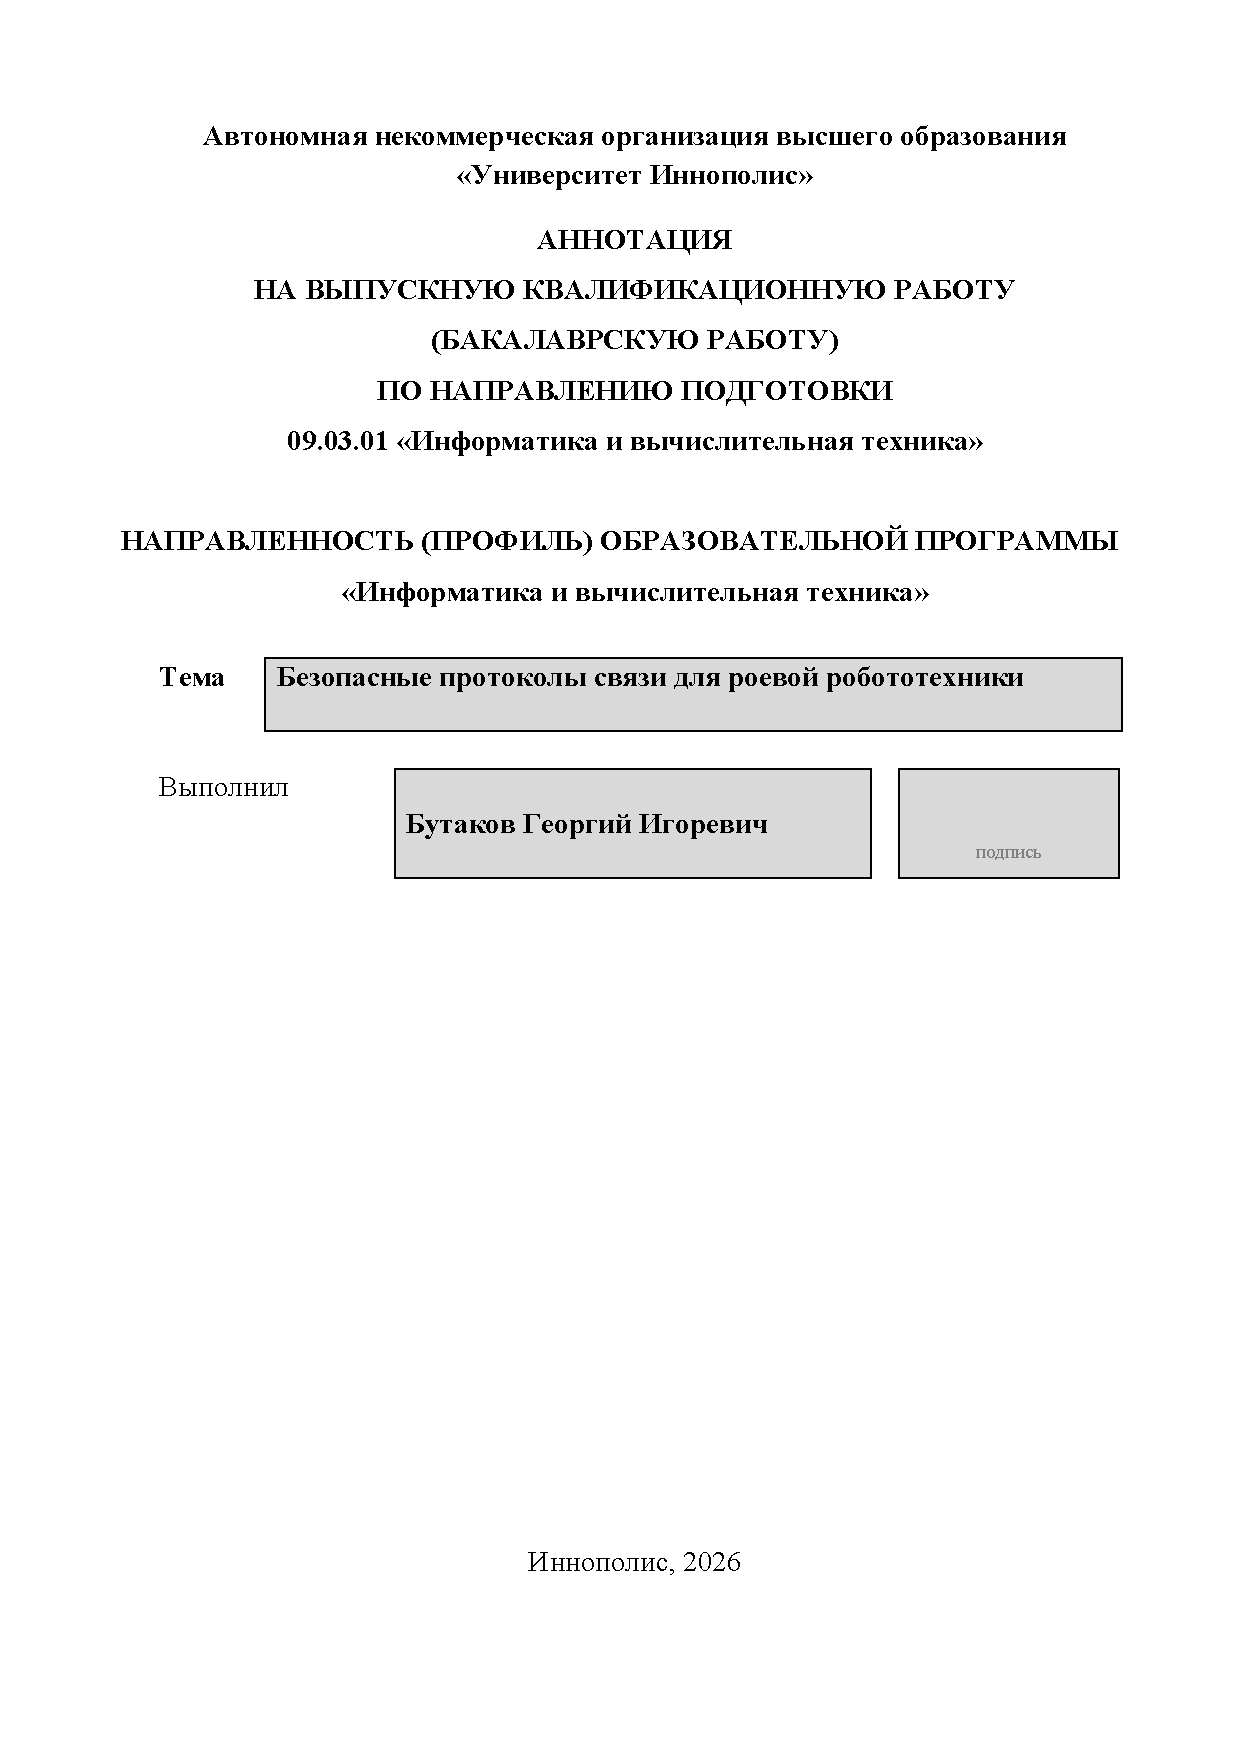
\includepdf[pages=-,pagecommand={\thispagestyle{empty}}]{annotation_title_page.pdf}
\setcounter{page}{2}

\tableofcontents
\newpage

\annotationsection{Введение}

Выпускная квалификационная работа посвящена разработке и оценке безопасных протоколов связи для роевой робототехники. Актуальность темы определяется тем, что рой автономных агентов зависит от постоянного обмена сообщениями, однако такие сообщения передаются по динамическим беспроводным каналам и обрабатываются устройствами с ограниченными вычислительными и энергетическими ресурсами. Поэтому фиксированный «тяжелый» криптографический режим может снижать пропускную способность и ускорять расход ресурсов, а постоянно облегченный режим может быть недостаточен при росте угрозы. Цель работы состоит в проектировании и экспериментальной оценке адаптивного облегченного фреймворка защищенной связи для \textenglish{swarm-oriented} систем. Объектом исследования является защищенная коммуникация в распределенных роевых системах, предметом -- адаптивный выбор криптографического профиля для защищенной \textenglish{data plane}. Научная новизна заключается в объединении формальной модели адаптивной связи с исполняемым прототипом, который позволяет измерить компромисс между уровнем защиты и стоимостью выполнения.

\annotationsection{Краткое описание основной части выпускной квалификационной работы}

В основной части работы выполнен обзор литературы по коммуникационным архитектурам роевых систем, легковесной криптографии, децентрализованному доверию и адаптивным подходам к безопасности. Анализ показывает, что существующие решения часто рассматривают связность, доверие и защиту сообщений раздельно. Поэтому в работе обоснована необходимость адаптивного подхода, который не фиксирует один криптографический профиль на всю миссию.

Теоретическая часть задает модель роя как динамического графа \(G(V,E,t)\), где вершины соответствуют агентам, а ребра описывают доступные каналы связи. На этой основе определяется функция адаптации \(F:S(t)\rightarrow P\), сопоставляющая состоянию системы набор параметров защиты. Модель угроз учитывает пассивное прослушивание, активное изменение и инъекцию сообщений, повторную передачу, подмену узла и отказ в обслуживании. Ключевыми требованиями к \textenglish{data plane} являются конфиденциальность, аутентификация, целостность и ограничение последствий компрометации через обновление ключевого материала.

Сравнение базовых протоколов показывает, что один примитив не решает всю задачу. X25519 используется для \textenglish{pairwise session establishment}, HKDF-SHA256 -- для вывода ключевого материала на эпоху, AEAD-схемы -- для защиты полезной нагрузки. AES-GCM применяется в \textenglish{heavy} и \textenglish{balanced} профилях, ChaCha20-Poly1305 -- в \textenglish{lightweight} профиле. Дополнительная runtime-аутентификация строится на HMAC-SHA256 или \textenglish{sequence-bound hash token}.

Практическая составляющая реализует три дискретных профиля и адаптивный выбор между ними. \textenglish{Heavy profile} использует AES-256-GCM и HMAC-SHA256; \textenglish{balanced profile} использует AES-192-GCM и HMAC-SHA256; \textenglish{lightweight profile} использует ChaCha20-Poly1305 и \textenglish{sequence-bound hash token}. Пороговая функция выбора усиливает защиту при \(\theta \geq 0.8\), переходит к облегченной защите при энергии ниже \(0.2E_{\max}\), а в остальных случаях выбирает \textenglish{balanced profile}.

Для проверки подхода реализован контейнерный \textenglish{benchmark} с двумя peer-узлами, соединенными через gRPC. Основная серия проводилась при ограничении 0.05 CPU core на узел, лимите памяти 128 MiB, размере сообщения 65\,536 bytes и продолжительности 60 seconds. Метрики включают latency, throughput, delivered-message count, drop rate, number of switches, profile mix, normalized energy proxy и cryptographic work per delivered message.

Результаты показывают, что при жестком CPU cap система достигает saturation между 25 и 75 messages per second. Наиболее устойчивым default оказался \textenglish{lightweight mode}: он показывает минимальную cryptographic work per delivered message, около 0.125 MiB, тогда как \textenglish{heavy} и \textenglish{balanced} обрабатывают около 0.250 MiB на доставленное сообщение из-за дополнительного HMAC pass. \textenglish{Adaptive mode} корректно переключается между профилями и располагается между статическими крайностями по эффективности.

\annotationsection{Заключение}

В результате работы разработан и экспериментально оценен адаптивный фреймворк защищенной связи для роевой робототехники. Основной вклад состоит в том, что формальная модель и архитектура были переведены в воспроизводимый \textenglish{pairwise prototype} с измеримыми режимами \textenglish{heavy}, \textenglish{balanced}, \textenglish{lightweight} и \textenglish{adaptive}. Полученные результаты подтверждают, что облегченный профиль является наиболее эффективным default при доминирующем вычислительном ограничении, а \textenglish{adaptive profile} полезен как policy-driven compromise. Выводы ограничены областью эксперимента: benchmark подтверждает поведение constrained host-based prototype, но не заменяет проверку на физических роботах, в large-swarm topology, при реальном sensing угроз и с полноценной authenticated control plane.

\annotationsection{Список использованной литературы}

\noindent 1. Dias P. G. F., Silva M. C., Rocha Filho G. P., Vargas P. A., Cota L. P., Pessin G. Swarm Robotics: A Perspective on the Latest Reviewed Concepts and Applications // Sensors. 2021. Vol. 21, No. 6. Article 2062.

\noindent 2. Debie E., Kasmarik K., Garratt M. Swarm Robotics: A Survey from a Multi-Tasking Perspective // ACM Computing Surveys. 2023. Vol. 56, No. 2. P. 1--38.

\noindent 3. Han P., Sui A., Wu J. Lightweight Secure Communication Supporting Batch Authentication for UAV Swarm // Drones. 2025. Vol. 9, No. 2. Article 139.

\noindent 4. Chen L., Ng S.-L. Securing Emergent Behaviour in Swarm Robotics // Journal of Information Security and Applications. 2022. Vol. 64. Article 103047.

\noindent 5. Adeniyi A. E., Jimoh R. G., Awotunde J. B. A Systematic Review on Elliptic Curve Cryptography Algorithm for Internet of Things // Computers and Electrical Engineering. 2024. Vol. 118. Article 109330.

\noindent 6. Manikandan K., Sriramulu R. ASMTP: Anonymous Secure Messaging Token-Based Protocol Assisted Data Security in Swarm of Unmanned Aerial Vehicles // International Journal of Network Management. 2024. Vol. 34, No. 6. Article e2271.

\noindent 7. RFC 7748. Elliptic Curves for Security. IRTF, 2016; RFC 8439. ChaCha20 and Poly1305 for IETF Protocols. IETF, 2018.

\end{document}
